% Created by tikzDevice version 0.10.1 on 2016-08-08 10:49:04
% !TEX encoding = UTF-8 Unicode
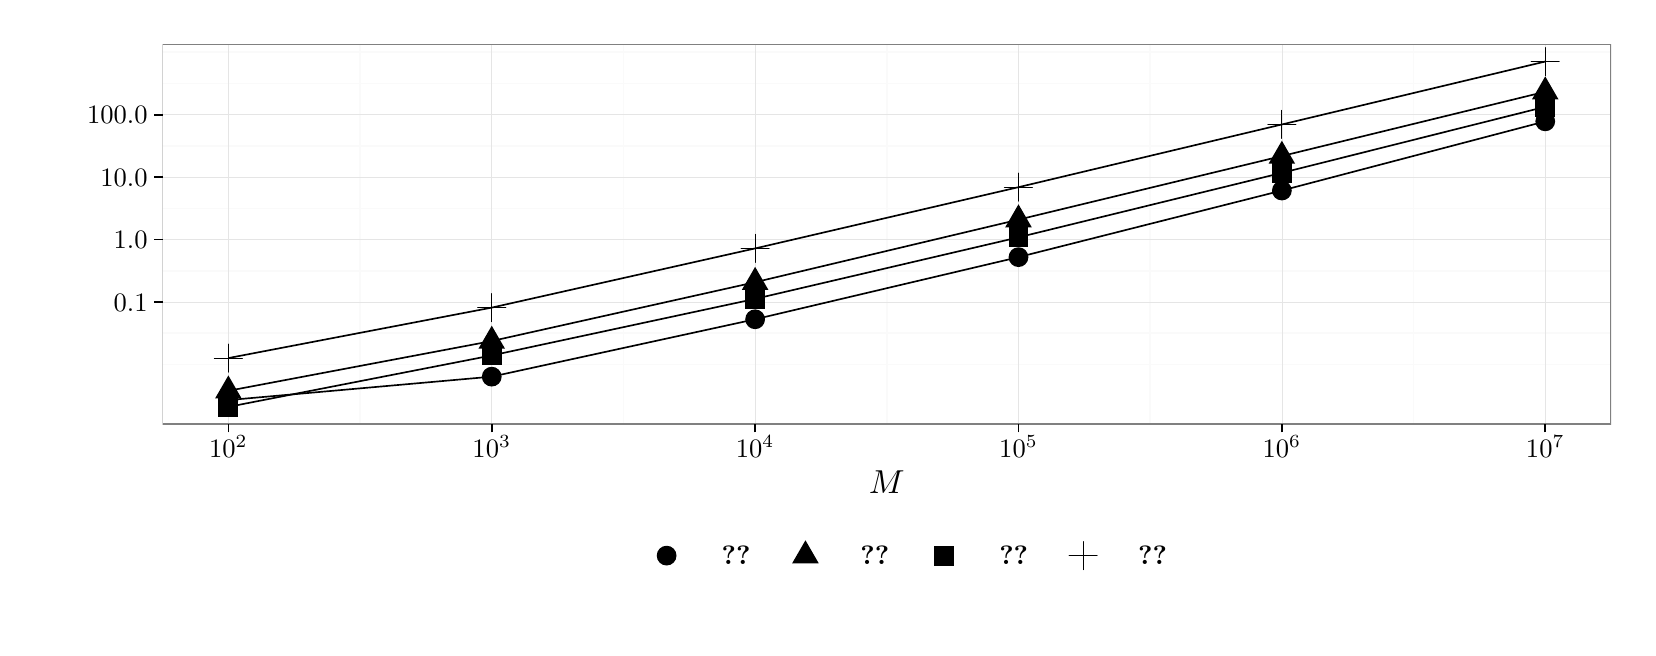
\begin{tikzpicture}[x=1pt,y=1pt]
\definecolor{fillColor}{RGB}{255,255,255}
\path[use as bounding box,fill=fillColor,fill opacity=0.00] (0,0) rectangle (578.16,216.81);
\begin{scope}
\path[clip] (  0.00,  0.00) rectangle (578.16,216.81);
\definecolor{drawColor}{RGB}{255,255,255}
\definecolor{fillColor}{RGB}{255,255,255}

\path[draw=drawColor,line width= 0.6pt,line join=round,line cap=round,fill=fillColor] (  0.00,  0.00) rectangle (578.16,216.81);
\end{scope}
\begin{scope}
\path[clip] ( 48.73, 73.54) rectangle (572.16,210.81);
\definecolor{fillColor}{RGB}{255,255,255}

\path[fill=fillColor] ( 48.73, 73.54) rectangle (572.16,210.81);
\definecolor{drawColor}{gray}{0.98}

\path[draw=drawColor,line width= 0.6pt,line join=round] ( 48.73, 95.07) --
	(572.16, 95.07);

\path[draw=drawColor,line width= 0.6pt,line join=round] ( 48.73,106.36) --
	(572.16,106.36);

\path[draw=drawColor,line width= 0.6pt,line join=round] ( 48.73,128.93) --
	(572.16,128.93);

\path[draw=drawColor,line width= 0.6pt,line join=round] ( 48.73,151.49) --
	(572.16,151.49);

\path[draw=drawColor,line width= 0.6pt,line join=round] ( 48.73,174.06) --
	(572.16,174.06);

\path[draw=drawColor,line width= 0.6pt,line join=round] ( 48.73,196.63) --
	(572.16,196.63);

\path[draw=drawColor,line width= 0.6pt,line join=round] ( 48.73,207.91) --
	(572.16,207.91);

\path[draw=drawColor,line width= 0.6pt,line join=round] (120.10, 73.54) --
	(120.10,210.81);

\path[draw=drawColor,line width= 0.6pt,line join=round] (215.27, 73.54) --
	(215.27,210.81);

\path[draw=drawColor,line width= 0.6pt,line join=round] (310.44, 73.54) --
	(310.44,210.81);

\path[draw=drawColor,line width= 0.6pt,line join=round] (405.61, 73.54) --
	(405.61,210.81);

\path[draw=drawColor,line width= 0.6pt,line join=round] (500.78, 73.54) --
	(500.78,210.81);
\definecolor{drawColor}{gray}{0.90}

\path[draw=drawColor,line width= 0.2pt,line join=round] ( 48.73,117.64) --
	(572.16,117.64);

\path[draw=drawColor,line width= 0.2pt,line join=round] ( 48.73,140.21) --
	(572.16,140.21);

\path[draw=drawColor,line width= 0.2pt,line join=round] ( 48.73,162.78) --
	(572.16,162.78);

\path[draw=drawColor,line width= 0.2pt,line join=round] ( 48.73,185.34) --
	(572.16,185.34);

\path[draw=drawColor,line width= 0.2pt,line join=round] ( 72.52, 73.54) --
	( 72.52,210.81);

\path[draw=drawColor,line width= 0.2pt,line join=round] (167.69, 73.54) --
	(167.69,210.81);

\path[draw=drawColor,line width= 0.2pt,line join=round] (262.86, 73.54) --
	(262.86,210.81);

\path[draw=drawColor,line width= 0.2pt,line join=round] (358.03, 73.54) --
	(358.03,210.81);

\path[draw=drawColor,line width= 0.2pt,line join=round] (453.20, 73.54) --
	(453.20,210.81);

\path[draw=drawColor,line width= 0.2pt,line join=round] (548.37, 73.54) --
	(548.37,210.81);
\definecolor{fillColor}{RGB}{0,0,0}

\path[fill=fillColor] ( 72.52, 82.24) circle (  3.57);

\path[fill=fillColor] (167.69, 90.70) circle (  3.57);

\path[fill=fillColor] (262.86,111.44) circle (  3.57);

\path[fill=fillColor] (358.03,133.89) circle (  3.57);

\path[fill=fillColor] (453.20,157.96) circle (  3.57);

\path[fill=fillColor] (548.37,182.95) circle (  3.57);

\path[fill=fillColor] ( 72.52, 91.14) --
	( 77.32, 82.82) --
	( 67.71, 82.82) --
	cycle;

\path[fill=fillColor] (167.69,109.12) --
	(172.49,100.80) --
	(162.88,100.80) --
	cycle;

\path[fill=fillColor] (262.86,130.38) --
	(267.66,122.06) --
	(258.05,122.06) --
	cycle;

\path[fill=fillColor] (358.03,152.99) --
	(362.83,144.66) --
	(353.22,144.66) --
	cycle;

\path[fill=fillColor] (453.20,175.97) --
	(458.00,167.65) --
	(448.39,167.65) --
	cycle;

\path[fill=fillColor] (548.37,199.21) --
	(553.17,190.88) --
	(543.56,190.88) --
	cycle;

\path[fill=fillColor] ( 68.95, 76.21) --
	( 76.09, 76.21) --
	( 76.09, 83.35) --
	( 68.95, 83.35) --
	cycle;

\path[fill=fillColor] (164.12, 94.80) --
	(171.26, 94.80) --
	(171.26,101.94) --
	(164.12,101.94) --
	cycle;

\path[fill=fillColor] (259.29,115.24) --
	(266.43,115.24) --
	(266.43,122.38) --
	(259.29,122.38) --
	cycle;

\path[fill=fillColor] (354.46,137.48) --
	(361.60,137.48) --
	(361.60,144.62) --
	(354.46,144.62) --
	cycle;

\path[fill=fillColor] (449.63,160.77) --
	(456.77,160.77) --
	(456.77,167.91) --
	(449.63,167.91) --
	cycle;

\path[fill=fillColor] (544.80,184.64) --
	(551.94,184.64) --
	(551.94,191.78) --
	(544.80,191.78) --
	cycle;
\definecolor{drawColor}{RGB}{0,0,0}

\path[draw=drawColor,line width= 0.4pt,line join=round,line cap=round] ( 67.47, 97.42) -- ( 77.57, 97.42);

\path[draw=drawColor,line width= 0.4pt,line join=round,line cap=round] ( 72.52, 92.37) -- ( 72.52,102.46);

\path[draw=drawColor,line width= 0.4pt,line join=round,line cap=round] (162.64,115.65) -- (172.74,115.65);

\path[draw=drawColor,line width= 0.4pt,line join=round,line cap=round] (167.69,110.60) -- (167.69,120.70);

\path[draw=drawColor,line width= 0.4pt,line join=round,line cap=round] (257.81,137.04) -- (267.90,137.04);

\path[draw=drawColor,line width= 0.4pt,line join=round,line cap=round] (262.86,131.99) -- (262.86,142.08);

\path[draw=drawColor,line width= 0.4pt,line join=round,line cap=round] (352.98,159.17) -- (363.07,159.17);

\path[draw=drawColor,line width= 0.4pt,line join=round,line cap=round] (358.03,154.12) -- (358.03,164.21);

\path[draw=drawColor,line width= 0.4pt,line join=round,line cap=round] (448.15,181.83) -- (458.24,181.83);

\path[draw=drawColor,line width= 0.4pt,line join=round,line cap=round] (453.20,176.78) -- (453.20,186.88);

\path[draw=drawColor,line width= 0.4pt,line join=round,line cap=round] (543.32,204.57) -- (553.41,204.57);

\path[draw=drawColor,line width= 0.4pt,line join=round,line cap=round] (548.37,199.52) -- (548.37,209.62);

\path[draw=drawColor,line width= 0.6pt,line join=round] ( 72.52, 82.24) --
	(167.69, 90.70) --
	(262.86,111.44) --
	(358.03,133.89) --
	(453.20,157.96) --
	(548.37,182.95);

\path[draw=drawColor,line width= 0.6pt,line join=round] ( 72.52, 85.59) --
	(167.69,103.57) --
	(262.86,124.83) --
	(358.03,147.44) --
	(453.20,170.42) --
	(548.37,193.66);

\path[draw=drawColor,line width= 0.6pt,line join=round] ( 72.52, 79.78) --
	(167.69, 98.37) --
	(262.86,118.81) --
	(358.03,141.05) --
	(453.20,164.34) --
	(548.37,188.21);

\path[draw=drawColor,line width= 0.6pt,line join=round] ( 72.52, 97.42) --
	(167.69,115.65) --
	(262.86,137.04) --
	(358.03,159.17) --
	(453.20,181.83) --
	(548.37,204.57);
\definecolor{drawColor}{gray}{0.50}

\path[draw=drawColor,line width= 0.6pt,line join=round,line cap=round] ( 48.73, 73.54) rectangle (572.16,210.81);
\end{scope}
\begin{scope}
\path[clip] (  0.00,  0.00) rectangle (578.16,216.81);
\definecolor{drawColor}{RGB}{0,0,0}

\node[text=drawColor,anchor=base east,inner sep=0pt, outer sep=0pt, scale=  0.96] at ( 43.33,114.34) {0.1};

\node[text=drawColor,anchor=base east,inner sep=0pt, outer sep=0pt, scale=  0.96] at ( 43.33,136.90) {1.0};

\node[text=drawColor,anchor=base east,inner sep=0pt, outer sep=0pt, scale=  0.96] at ( 43.33,159.47) {10.0};

\node[text=drawColor,anchor=base east,inner sep=0pt, outer sep=0pt, scale=  0.96] at ( 43.33,182.04) {100.0};
\end{scope}
\begin{scope}
\path[clip] (  0.00,  0.00) rectangle (578.16,216.81);
\definecolor{drawColor}{RGB}{0,0,0}

\path[draw=drawColor,line width= 0.6pt,line join=round] ( 45.73,117.64) --
	( 48.73,117.64);

\path[draw=drawColor,line width= 0.6pt,line join=round] ( 45.73,140.21) --
	( 48.73,140.21);

\path[draw=drawColor,line width= 0.6pt,line join=round] ( 45.73,162.78) --
	( 48.73,162.78);

\path[draw=drawColor,line width= 0.6pt,line join=round] ( 45.73,185.34) --
	( 48.73,185.34);
\end{scope}
\begin{scope}
\path[clip] (  0.00,  0.00) rectangle (578.16,216.81);
\definecolor{drawColor}{RGB}{0,0,0}

\path[draw=drawColor,line width= 0.6pt,line join=round] ( 72.52, 70.54) --
	( 72.52, 73.54);

\path[draw=drawColor,line width= 0.6pt,line join=round] (167.69, 70.54) --
	(167.69, 73.54);

\path[draw=drawColor,line width= 0.6pt,line join=round] (262.86, 70.54) --
	(262.86, 73.54);

\path[draw=drawColor,line width= 0.6pt,line join=round] (358.03, 70.54) --
	(358.03, 73.54);

\path[draw=drawColor,line width= 0.6pt,line join=round] (453.20, 70.54) --
	(453.20, 73.54);

\path[draw=drawColor,line width= 0.6pt,line join=round] (548.37, 70.54) --
	(548.37, 73.54);
\end{scope}
\begin{scope}
\path[clip] (  0.00,  0.00) rectangle (578.16,216.81);
\definecolor{drawColor}{RGB}{0,0,0}

\node[text=drawColor,anchor=base,inner sep=0pt, outer sep=0pt, scale=  0.96] at ( 72.52, 61.53) {$10^{2}$};

\node[text=drawColor,anchor=base,inner sep=0pt, outer sep=0pt, scale=  0.96] at (167.69, 61.53) {$10^{3}$};

\node[text=drawColor,anchor=base,inner sep=0pt, outer sep=0pt, scale=  0.96] at (262.86, 61.53) {$10^{4}$};

\node[text=drawColor,anchor=base,inner sep=0pt, outer sep=0pt, scale=  0.96] at (358.03, 61.53) {$10^{5}$};

\node[text=drawColor,anchor=base,inner sep=0pt, outer sep=0pt, scale=  0.96] at (453.20, 61.53) {$10^{6}$};

\node[text=drawColor,anchor=base,inner sep=0pt, outer sep=0pt, scale=  0.96] at (548.37, 61.53) {$10^{7}$};
\end{scope}
\begin{scope}
\path[clip] (  0.00,  0.00) rectangle (578.16,216.81);
\definecolor{drawColor}{RGB}{0,0,0}

\node[text=drawColor,anchor=base,inner sep=0pt, outer sep=0pt, scale=  1.20] at (310.44, 48.46) {$M$};
\end{scope}
\begin{scope}
\path[clip] (  0.00,  0.00) rectangle (578.16,216.81);
\definecolor{fillColor}{RGB}{255,255,255}

\path[fill=fillColor] (204.93, 14.54) rectangle (415.96, 37.53);
\end{scope}
\begin{scope}
\path[clip] (  0.00,  0.00) rectangle (578.16,216.81);
\definecolor{fillColor}{RGB}{255,255,255}

\path[fill=fillColor] (212.81, 18.80) rectangle (248.94, 33.26);
\end{scope}
\begin{scope}
\path[clip] (  0.00,  0.00) rectangle (578.16,216.81);
\definecolor{fillColor}{RGB}{0,0,0}

\path[fill=fillColor] (230.88, 26.03) circle (  3.57);
\end{scope}
\begin{scope}
\path[clip] (  0.00,  0.00) rectangle (578.16,216.81);
\definecolor{fillColor}{RGB}{255,255,255}

\path[fill=fillColor] (262.98, 18.80) rectangle (299.12, 33.26);
\end{scope}
\begin{scope}
\path[clip] (  0.00,  0.00) rectangle (578.16,216.81);
\definecolor{fillColor}{RGB}{0,0,0}

\path[fill=fillColor] (281.05, 31.58) --
	(285.85, 23.26) --
	(276.24, 23.26) --
	cycle;
\end{scope}
\begin{scope}
\path[clip] (  0.00,  0.00) rectangle (578.16,216.81);
\definecolor{fillColor}{RGB}{255,255,255}

\path[fill=fillColor] (313.15, 18.80) rectangle (349.29, 33.26);
\end{scope}
\begin{scope}
\path[clip] (  0.00,  0.00) rectangle (578.16,216.81);
\definecolor{fillColor}{RGB}{0,0,0}

\path[fill=fillColor] (327.65, 22.46) --
	(334.79, 22.46) --
	(334.79, 29.60) --
	(327.65, 29.60) --
	cycle;
\end{scope}
\begin{scope}
\path[clip] (  0.00,  0.00) rectangle (578.16,216.81);
\definecolor{fillColor}{RGB}{255,255,255}

\path[fill=fillColor] (363.33, 18.80) rectangle (399.46, 33.26);
\end{scope}
\begin{scope}
\path[clip] (  0.00,  0.00) rectangle (578.16,216.81);
\definecolor{drawColor}{RGB}{0,0,0}

\path[draw=drawColor,line width= 0.4pt,line join=round,line cap=round] (376.35, 26.03) -- (386.44, 26.03);

\path[draw=drawColor,line width= 0.4pt,line join=round,line cap=round] (381.39, 20.98) -- (381.39, 31.08);
\end{scope}
\begin{scope}
\path[clip] (  0.00,  0.00) rectangle (578.16,216.81);
\definecolor{drawColor}{RGB}{0,0,0}

\node[text=drawColor,anchor=base east,inner sep=0pt, outer sep=0pt, scale=  0.96] at (261.17, 22.72) {\ref{Scen:change_in_mean}};
\end{scope}
\begin{scope}
\path[clip] (  0.00,  0.00) rectangle (578.16,216.81);
\definecolor{drawColor}{RGB}{0,0,0}

\node[text=drawColor,anchor=base east,inner sep=0pt, outer sep=0pt, scale=  0.96] at (311.35, 22.72) {\ref{Scen:change_in_slope}};
\end{scope}
\begin{scope}
\path[clip] (  0.00,  0.00) rectangle (578.16,216.81);
\definecolor{drawColor}{RGB}{0,0,0}

\node[text=drawColor,anchor=base east,inner sep=0pt, outer sep=0pt, scale=  0.96] at (361.52, 22.72) {\ref{Scen:change_in_mean_and_slope}};
\end{scope}
\begin{scope}
\path[clip] (  0.00,  0.00) rectangle (578.16,216.81);
\definecolor{drawColor}{RGB}{0,0,0}

\node[text=drawColor,anchor=base east,inner sep=0pt, outer sep=0pt, scale=  0.96] at (411.69, 22.72) {\ref{Scen:change_in_mean_and_variance}};
\end{scope}
\end{tikzpicture}
